\HydraSection[
  focus x=0.62,
  focus y=0.44,
  radius=0.12,
  zoom=1.90
]{Gierer--Meinhardt model}


\begin{frame}{Return to the Gierer--Meinhardt model}

  \vspace{-0.38cm}

  \begin{columns}[c,onlytextwidth]

    \begin{column}{0.60\textwidth}

      {\color{HydraWhite}\fontsize{8.4}{10.3}\selectfont
        Let $\Omega\subset\mathbb R^n$ be a bounded domain
      \par}

      \vspace{-0.28cm}

      {\color{HydraWhite}\fontsize{9.7}{12.3}\selectfont
      \begin{align*}
        \begin{aligned}
          \partial_tu
          &=
          D_u\Delta u+\frac{au^2}{K+v}-\mu_u u
          \\
          \partial_tv
          &=
          D_v\Delta v+bu^2-\mu_v v
        \end{aligned}
      \end{align*}
      }

      \vspace{-0.42cm}

      {\color{HydraWhite}\fontsize{8.4}{10.3}\selectfont
        Initial conditions
      \par}

      \vspace{-0.50cm}

      {\color{HydraWhite}\fontsize{8.9}{11.3}\selectfont
      \begin{align*}
        u(x,0)&=u_0(x)
        &
        v(x,0)&=v_0(x)
        &&x\in\Omega
      \end{align*}
      }

      \vspace{-0.46cm}

      {\color{HydraWhite}\fontsize{8.4}{10.3}\selectfont
        Homogeneous Neumann boundary conditions
      \par}

      \vspace{-0.50cm}

      {\color{HydraWhite}\fontsize{8.9}{11.3}\selectfont
      \begin{align*}
        \nabla u\cdot\mathbf n
        &=0
        &
        \nabla v\cdot\mathbf n
        &=0
        &&x\in\partial\Omega
      \end{align*}
      }

    \end{column}

    \begin{column}{0.36\textwidth}
      \vspace{0.8cm}
      \HydraPoint[HydraGold]
        {Homogeneous states}
        {Which constant concentrations can persist in time?}

      \vspace{-0.09cm}

      \HydraPoint[HydraCyan]
        {Local stability}
        {Which states recover after a spatially uniform perturbation?}

      \vspace{-0.09cm}

      \HydraPoint[HydraGold]
        {Diffusion-driven instability}
        {Can diffusion destabilize a locally stable active state?}

    \end{column}

  \end{columns}

  \vspace{0.42cm}

  {\color{HydraWhite}\fontsize{7.2}{8.9}\selectfont
  \begin{columns}[T,onlytextwidth]

    \begin{column}{0.31\textwidth}
      \textcolor{HydraGold}{$u$}\quad activator concentration

      \vspace{0.10cm}

      \textcolor{HydraCyan}{$v$}\quad inhibitor concentration
    \end{column}

    \begin{column}{0.31\textwidth}
      \textcolor{HydraCyan}{$D_u,D_v$}\quad diffusion coefficients

      \vspace{0.10cm}

      \textcolor{HydraGold}{$a$}\quad activator self-amplification

      \vspace{0.10cm}

      \textcolor{HydraGold}{$K$}\quad inhibition scale
    \end{column}

    \begin{column}{0.31\textwidth}
      \textcolor{HydraGold}{$b$}\quad inhibitor production

      \vspace{0.10cm}

      \textcolor{HydraWhite}{$\mu_u,\mu_v$}\quad degradation rates
    \end{column}

  \end{columns}
  }

\end{frame}


\HydraSubsection[
  \mbox{The geometry of the local reactions}
  \mbox{reveals an activation threshold}
  \mbox{and two competing stable outcomes}
]{Steady states}


\begin{frame}{Reaction system}

  \vspace{-0.20cm}

  {\color{HydraMuted}\fontsize{8.2}{10.1}\selectfont
    Looking for steady states and analyzing stability
  \par}

  \vspace{-0.06cm}

  \begin{columns}[T,onlytextwidth]

    \begin{column}{0.54\textwidth}


      \vspace{-0.18cm}

      {\color{HydraWhite}\fontsize{10.8}{13.8}\selectfont
      \begin{align*}
        \partial_tu
        &=
        f(u,v)
        =
        \frac{au^2}{K+v}-\mu_u u
        \\
        \partial_tv
        &=
        g(u,v)
        =
        bu^2-\mu_v v
      \end{align*}
      }

      \vspace{-0.30cm}

      {\color{HydraMuted}\fontsize{7.7}{9.5}\selectfont
        Without diffusion every spatial position follows the same two-variable reaction system
      \par}

    \end{column}

    \begin{column}{0.42\textwidth}

      \HydraPoint[HydraGold]
        {Steady states}
        {Find constant concentrations $(\bar u,\bar v)$ for which $f(\bar u,\bar v)=0$ and $g(\bar u,\bar v)=0$}

      \vspace{-0.00cm}

      \HydraPoint[HydraCyan]
        {Local stability}
        {Linearize the reaction system around each steady state and inspect the eigenvalues of the Jacobian}

    \end{column}

  \end{columns}

\end{frame}


\begin{frame}{Steady states}

  \vspace{-0.18cm}

  \begin{columns}[c,onlytextwidth]

    \begin{column}{0.47\textwidth}

      {\color{HydraMuted}\fontsize{7.8}{9.6}\selectfont
        A homogeneous steady state $(\bar u,\bar v)$ satisfies
      \par}

      \vspace{-0.18cm}

      {\color{HydraWhite}\fontsize{9.7}{12.3}\selectfont
      \begin{align*}
        0
        &=
        \frac{a\bar u^2}{K+\bar v}-\mu_u\bar u
        \\
        0
        &=
        b\bar u^2-\mu_v\bar v
      \end{align*}
      }

      \vspace{-0.34cm}

      {\color{HydraMuted}\fontsize{7.8}{9.6}\selectfont
        The second equation gives
      \par}

      \vspace{-0.24cm}

      {\color{HydraWhite}\bfseries\fontsize{11}{13.8}\selectfont
      \begin{align*}
        \bar v
        &=
        \frac{b}{\mu_v}\bar u^2
      \end{align*}
      }

    \end{column}

    \begin{column}{0.49\textwidth}

      {\color{HydraMuted}\fontsize{7.8}{9.6}\selectfont
        Substitution into the first equation gives
      \par}

      \vspace{-0.18cm}

      {\color{HydraWhite}\fontsize{9.2}{11.7}\selectfont
      \begin{align*}
        0
        &=
        \frac{a\bar u^2}
        {K+\frac{b}{\mu_v}\bar u^2}
        -
        \mu_u\bar u
      \end{align*}
      }

      \vspace{-0.34cm}

      {\color{HydraMuted}\fontsize{7.8}{9.6}\selectfont
        After clearing the denominator
      \par}

      \vspace{-0.22cm}

      {\color{HydraGold}\bfseries\fontsize{10.3}{13}\selectfont
      \begin{align*}
        \boxed{
          \bar u
          \left(
            \frac{b}{\mu_v}\bar u^2
            -
            \frac{a}{\mu_u}\bar u
            +
            K
          \right)
          =
          0
        }
      \end{align*}
      }

    \end{column}

  \end{columns}

  \vspace{-0.12cm}

  \HydraTakeaway{
    A cubic equation determines all homogeneous steady states
  }

\end{frame}


\begin{frame}{Steady states: two positive roots}

  \vspace{-0.16cm}

  \begin{center}
    {\color{HydraWhite}\fontsize{11.2}{14.2}\selectfont
    \begin{align*}
      \bar u=0
      &\quad\Rightarrow\quad
      (\bar u,\bar v)=(0,0)
      \\
      \bar u>0
      &\quad\Rightarrow\quad
      \frac{b}{\mu_v}\bar u^2
      -
      \frac{a}{\mu_u}\bar u
      +
      K
      =
      0
    \end{align*}
    }
  \end{center}

  \vspace{-0.20cm}

  \begin{columns}[c,onlytextwidth]
    \begin{column}{0.64\textwidth}
      {\color{HydraGold}\bfseries\fontsize{7.7}{9.2}\selectfont
        TWO POSITIVE STEADY STATES IF
        \(\boldsymbol{a^2\mu_v>4bK\mu_u^2}\)\par}

      \vspace{-0.20cm}

      {\color{HydraWhite}\fontsize{10.6}{13.5}\selectfont
      \[
        u_\pm=\frac{\mu_v}{2b}
        \left[
          \frac{a}{\mu_u}
          \pm
          \sqrt{
            \left(\frac{a}{\mu_u}\right)^2
            -\frac{4bK}{\mu_v}
          }
        \right]
      \]
      }

      \vspace{-0.24cm}

      {\color{HydraWhite}\fontsize{10.8}{13.6}\selectfont
      \[
        v_\pm=\frac{b}{\mu_v}u_\pm^2
      \]
      }
    \end{column}

    \begin{column}{0.32\textwidth}
      \HydraPoint[HydraRed]
        {Lower state $(u_-,v_-)$}
        {The smaller positive root will become the activation threshold}

      \vspace{-0.00cm}

      \HydraPoint[HydraGreen]
        {Upper state $(u_+,v_+)$}
        {The larger positive root is the candidate active state}
    \end{column}
  \end{columns}

  \vspace{-0.12cm}

  \HydraTakeaway{
    The nonlinear reaction terms can create two distinct positive concentration levels
  }
\end{frame}


\begin{frame}{The nullclines}

  \vspace{-0.12cm}

  \begin{columns}[c,onlytextwidth]
    \begin{column}{0.44\textwidth}
      {\color{HydraGold}\bfseries\fontsize{7.6}{9.1}\selectfont
        ACTIVATOR NULLCLINE\par}

      \vspace{-0.18cm}

      {\color{HydraWhite}\fontsize{10.1}{13.1}\selectfont
      \begin{align*}
        f(u,v)
        &=
        \frac{au^2}{K+v}-\mu_u u
        =
        0
        \\
        &\iff
        u=0
        \quad\text{or}\quad
        v=\frac{a}{\mu_u}u-K
      \end{align*}
      }

      \vspace{-0.18cm}

      {\color{HydraCyan}\bfseries\fontsize{7.6}{9.1}\selectfont
        INHIBITOR NULLCLINE\par}

      \vspace{-0.18cm}

      {\color{HydraWhite}\fontsize{10.1}{13.1}\selectfont
      \begin{align*}
        g(u,v)
        &=
        bu^2-\mu_v v
        =
        0
        \\
        &\iff
        v=\frac{b}{\mu_v}u^2
      \end{align*}
      }

      \vspace{-0.12cm}

      {\color{HydraMuted}\fontsize{7.6}{9.5}\selectfont
        Positive equilibria are intersections of a straight line and a parabola
      \par}
    \end{column}

    \begin{column}{0.52\textwidth}
      \centering

      % REPLACEABLE VISUAL
      % Replace the tikzpicture with:
      % \includegraphics[width=\linewidth,height=5.25cm,keepaspectratio]{figures/D_gierer_meinhardt/nullclines.png}
      \begin{tikzpicture}[x=0.92cm,y=0.92cm]
        \draw[-{Latex[length=2.2mm]},HydraMuted,line width=0.75pt]
          (0.25,0.55) -- (6.05,0.55)
          node[below,text=HydraMuted,font=\fontsize{7}{8.2}\selectfont] {$u$};
        \draw[-{Latex[length=2.2mm]},HydraMuted,line width=0.75pt]
          (0.55,0.25) -- (0.55,5.35)
          node[left,text=HydraMuted,font=\fontsize{7}{8.2}\selectfont] {$v$};

        \begin{scope}
          \clip (0.55,0.55) rectangle (5.75,5.15);

          \draw[HydraCyan,line width=1.75pt,domain=0.55:4.85,samples=100]
            plot (\x,{0.55+0.25*(\x-0.55)*(\x-0.55)});

          \draw[HydraGold,line width=1.75pt]
            (1.25,0.55) -- (5.25,4.95);

          \draw[HydraGold,line width=1.75pt]
            (0.55,0.55) -- (0.55,5.15);
        \end{scope}

        \fill[HydraWhite] (0.55,0.55) circle[radius=0.075cm];
        \fill[HydraRed] (1.42,0.74) circle[radius=0.080cm];
        \fill[HydraGreen] (4.08,3.66) circle[radius=0.080cm];

        \node[anchor=north west,text=HydraWhite,
          font=\bfseries\fontsize{6.7}{8.1}\selectfont]
          at (0.65,0.48) {$(0,0)$};
        \node[anchor=north west,text=HydraRed,
          font=\bfseries\fontsize{6.7}{8.1}\selectfont]
          at (1.52,0.65) {$(u_-,v_-)$};
        \node[anchor=north west,text=HydraGreen,
          font=\bfseries\fontsize{6.7}{8.1}\selectfont]
          at (4.18,3.52) {$(u_+,v_+)$};

        \node[anchor=west,text=HydraCyan,
          font=\bfseries\fontsize{7}{8.5}\selectfont]
          at (2.72,1.24) {$g(u,v)=0$};
        \node[anchor=west,text=HydraGold,
          font=\bfseries\fontsize{7}{8.5}\selectfont]
          at (1.34,3.18) {$f(u,v)=0$};
        \node[text=HydraGold,rotate=90,
          font=\fontsize{6.6}{8}\selectfont]
          at (0.88,4.45) {$u=0$};
      \end{tikzpicture}
    \end{column}
  \end{columns}
\end{frame}


\begin{frame}{Possible steady states}

  \vspace{-0.13cm}

  \begin{columns}[c,onlytextwidth]
    \begin{column}{0.34\textwidth}
      {\color{HydraGold}\bfseries\fontsize{7.5}{9}\selectfont
        EXISTENCE CONDITION\par}

      \vspace{-0.16cm}

      {\color{HydraWhite}\bfseries\fontsize{10.5}{13.5}\selectfont
      \begin{align*}
        \boxed{
          \left(\frac{a}{\mu_u}\right)^2
          >\frac{4bK}{\mu_v}
        }
      \end{align*}
      }

      \vspace{-0.20cm}

      {\color{HydraMuted}\fontsize{7.4}{9.2}\selectfont
        At equality, the line is tangent to the parabola and the two positive equilibria merge
      \par}
    \end{column}

    \begin{column}{0.62\textwidth}
      \centering

      % REPLACEABLE VISUAL
      % Replace the tikzpicture with:
      % \includegraphics[width=\linewidth,height=4.95cm,keepaspectratio]{figures/D_gierer_meinhardt/saddle_node.png}
      \begin{tikzpicture}[x=0.62cm,y=0.62cm]

        % No positive steady state
        \begin{scope}[xshift=0cm]
          \node[text=HydraMuted,font=\bfseries\fontsize{6.3}{7.6}\selectfont]
            at (1.95,3.92) {NO POSITIVE STATE};

          \draw[-{Latex[length=1.8mm]},HydraMuted,line width=0.65pt]
            (0.20,0.35) -- (3.75,0.35);
          \draw[-{Latex[length=1.8mm]},HydraMuted,line width=0.65pt]
            (0.35,0.20) -- (0.35,3.55);

          \draw[HydraCyan,line width=1.25pt,domain=0.35:3.45,samples=75]
            plot (\x,{0.35+0.28*(\x-0.35)*(\x-0.35)});
          \draw[HydraGold,line width=1.25pt]
            (1.00,0.35) -- (3.45,1.38);
          \draw[HydraGold,line width=1.25pt]
            (0.35,0.35) -- (0.35,3.45);

          \fill[HydraWhite] (0.35,0.35) circle[radius=0.070cm];

          \node[text=HydraWhite,font=\bfseries\fontsize{6.2}{7.5}\selectfont]
            at (1.95,-0.18) {1 steady state};
          \node[text=HydraMuted,font=\fontsize{6.2}{7.5}\selectfont]
            at (1.95,-0.55) {$(0,0)$};
        \end{scope}

        % Saddle-node tangency
        \begin{scope}[xshift=3.25cm]
          \node[text=HydraGold,font=\bfseries\fontsize{6.3}{7.6}\selectfont]
            at (1.95,3.92) {TANGENCY};

          \draw[-{Latex[length=1.8mm]},HydraMuted,line width=0.65pt]
            (0.20,0.35) -- (3.75,0.35);
          \draw[-{Latex[length=1.8mm]},HydraMuted,line width=0.65pt]
            (0.35,0.20) -- (0.35,3.55);

          \draw[HydraCyan,line width=1.25pt,domain=0.35:3.45,samples=75]
            plot (\x,{0.35+0.28*(\x-0.35)*(\x-0.35)});
          \draw[HydraGold,line width=1.25pt]
            (1.00,0.35) -- (3.45,2.13);
          \draw[HydraGold,line width=1.25pt]
            (0.35,0.35) -- (0.35,3.45);

          \fill[HydraWhite] (0.35,0.35) circle[radius=0.070cm];
          \fill[HydraGold] (1.65,0.82) circle[radius=0.075cm];

          \node[text=HydraWhite,font=\bfseries\fontsize{6.2}{7.5}\selectfont]
            at (1.95,-0.18) {2 steady states};
          \node[text=HydraMuted,font=\fontsize{5.8}{7}\selectfont]
            at (1.95,-0.55) {$(0,0)\quad (u_c,v_c)$};
        \end{scope}

        % Two positive steady states
        \begin{scope}[xshift=6.50cm]
          \node[text=HydraCyan,font=\bfseries\fontsize{6.3}{7.6}\selectfont]
            at (1.95,3.92) {TWO POSITIVE STATES};

          \draw[-{Latex[length=1.8mm]},HydraMuted,line width=0.65pt]
            (0.20,0.35) -- (3.75,0.35);
          \draw[-{Latex[length=1.8mm]},HydraMuted,line width=0.65pt]
            (0.35,0.20) -- (0.35,3.55);

          \draw[HydraCyan,line width=1.25pt,domain=0.35:3.45,samples=75]
            plot (\x,{0.35+0.28*(\x-0.35)*(\x-0.35)});
          \draw[HydraGold,line width=1.25pt]
            (1.00,0.35) -- (3.45,2.68);
          \draw[HydraGold,line width=1.25pt]
            (0.35,0.35) -- (0.35,3.45);

          \fill[HydraWhite] (0.35,0.35) circle[radius=0.070cm];
          \fill[HydraRed] (1.23,0.57) circle[radius=0.075cm];
          \fill[HydraGreen] (2.87,2.12) circle[radius=0.075cm];

          \node[text=HydraWhite,font=\bfseries\fontsize{6.2}{7.5}\selectfont]
            at (1.95,-0.18) {3 steady states};
          \node[text=HydraMuted,font=\fontsize{5.3}{6.5}\selectfont]
            at (1.95,-0.55)
            {$(0,0)\quad (u_-,v_-)\quad (u_+,v_+)$};
        \end{scope}

      \end{tikzpicture}
    \end{column}
  \end{columns}

  \vspace{0.58cm}

  \HydraTakeaway{
    Strong enough autocatalysis creates the zero state and two positive states separated by a threshold
  }
\end{frame}


\HydraSubsection[
  \mbox{We first analyse stability in the local}
  \mbox{reaction system without diffusion}
  \mbox{and identify the activation threshold}
]{Local stability}


\begin{frame}{The zero steady state is always stable}

  \vspace{-0.30cm}

  \begin{columns}[c,onlytextwidth]

    \begin{column}{0.60\textwidth}


      \vspace{-0.30cm}

      {\color{HydraWhite}\fontsize{8.6}{10.9}\selectfont
      \begin{align*}
        f(u,v)
        &=
        \frac{au^2}{K+v}-\mu_u u
        &
        g(u,v)
        &=
        bu^2-\mu_v v
      \end{align*}
      }

      \vspace{-0.46cm}

      {\color{HydraGold}\bfseries\fontsize{7.5}{9}\selectfont
        JACOBIAN\par}

      \vspace{-0.30cm}

      {\color{HydraWhite}\fontsize{8.3}{10.6}\selectfont
      \begin{align*}
        J(u,v)
        &=
        \begin{pmatrix}
          f_u(u,v)&f_v(u,v)
          \\
          g_u(u,v)&g_v(u,v)
        \end{pmatrix}
        \\
        &=
        \begin{pmatrix}
          \dfrac{2au}{K+v}-\mu_u
          &
          -\dfrac{au^2}{(K+v)^2}
          \\[0.14cm]
          2bu
          &
          -\mu_v
        \end{pmatrix}
      \end{align*}
      }

      \vspace{-0.50cm}

      {\color{HydraWhite}\fontsize{9.4}{12}\selectfont
      \begin{align*}
        J(0,0)
        &=
        \begin{pmatrix}
          -\mu_u&0
          \\
          0&-\mu_v
        \end{pmatrix}
        ,
        &
        \begin{aligned}
          \lambda_1&=-\mu_u<0
          \\
          \lambda_2&=-\mu_v<0
        \end{aligned}
      \end{align*}
      }

      \vspace{-0.34cm}

      \HydraPoint[HydraGold]
        {Asymptotically stable}
        {Near $u=0$ quadratic activator production is dominated by linear degradation}

    \end{column}

    \begin{column}{0.36\textwidth}
      \centering

      % REPLACEABLE VISUAL
      % Replace the tikzpicture with:
      % \includegraphics[width=\linewidth,height=4.85cm,keepaspectratio]{figures/D_gierer_meinhardt/origin_stability.png}
      \begin{tikzpicture}[x=0.88cm,y=0.88cm]
        \coordinate (O) at (0.55,0.55);

        \draw[-{Latex[length=2mm]},HydraMuted,line width=0.7pt]
          (0.40,0.55) -- (5.20,0.55)
          node[below,text=HydraMuted,font=\fontsize{7}{8.2}\selectfont] {$u$};
        \draw[-{Latex[length=2mm]},HydraMuted,line width=0.7pt]
          (0.55,0.40) -- (0.55,4.95)
          node[left,text=HydraMuted,font=\fontsize{7}{8.2}\selectfont] {$v$};

        \foreach \x in {1.15,1.95,2.75,3.55,4.35}{
          \foreach \y in {1.10,1.90,2.70,3.50,4.30}{
            \pgfmathsetmacro{\vx}{0.55-\x}
            \pgfmathsetmacro{\vy}{0.55-\y}
            \pgfmathsetmacro{\vn}{sqrt(\vx*\vx+\vy*\vy)}
            \pgfmathsetmacro{\dx}{0.34*\vx/\vn}
            \pgfmathsetmacro{\dy}{0.34*\vy/\vn}
            \draw[-{Latex[length=1.55mm]},HydraCyan,line width=0.72pt]
              (\x,\y) -- ++(\dx,\dy);
          }
        }

        \fill[HydraGreen] (O) circle[radius=0.090cm];
        \node[anchor=south west,text=HydraGreen,
          font=\bfseries\fontsize{7.2}{8.6}\selectfont]
          at (0.70,0.00) {$(0,0)$};

        \node[text=HydraMuted,font=\fontsize{7}{8.5}\selectfont,
          align=center,text width=3.5cm]
          at (3.15,4.72) {nearby trajectories return to $(0,0)$};
      \end{tikzpicture}

    \end{column}

  \end{columns}

\end{frame}


\begin{frame}{Jacobian at the positive steady states}

  \vspace{-0.26cm}

  {\color{HydraMuted}\fontsize{7.8}{9.6}\selectfont
    At either positive steady state $(u_\pm,v_\pm)$ the activator equation gives
  \par}

  \vspace{-0.30cm}

  {\color{HydraWhite}\fontsize{9.6}{12.1}\selectfont
  \begin{align*}
    f(u_\pm,v_\pm)
    =
    \frac{au_\pm^2}{K+v_\pm}
    -
    \mu_u u_\pm
    =
    0
    \qquad\Rightarrow\qquad
    \frac{au_\pm}{K+v_\pm}
    =
    \mu_u
  \end{align*}
  }

  \vspace{-0.42cm}

  \begin{columns}[T,onlytextwidth]

    \begin{column}{0.48\textwidth}
      {\centering
      {\color{HydraGold}\bfseries\fontsize{7.5}{9}\selectfont
         ACTIVATOR DERIVATIVES\par}
      }

      \vspace{-0.28cm}

      {\color{HydraWhite}\fontsize{8.7}{11}\selectfont
      \begin{align*}
        f_u(u_\pm,v_\pm)
        &=
        \frac{2au_\pm}{K+v_\pm}-\mu_u
        =
        \mu_u
        \\
        f_v(u_\pm,v_\pm)
        &=
        -\frac{au_\pm^2}{(K+v_\pm)^2}
        =
        -\frac{\mu_u^2}{a}
      \end{align*}
      }

    \end{column}

    \begin{column}{0.48\textwidth}
      {\centering
      {\color{HydraCyan}\bfseries\fontsize{7.5}{9}\selectfont
         INHIBITOR DERIVATIVES\par}
         }

      \vspace{-0.28cm}

      {\color{HydraWhite}\fontsize{8.7}{11}\selectfont
      \begin{align*}
        g_u(u_\pm,v_\pm)
        &=
        2bu_\pm
        \\
        g_v(u_\pm,v_\pm)
        &=
        -\mu_v
      \end{align*}
      }

    \end{column}

  \end{columns}

  \vspace{-0.34cm}

  {\color{HydraGold}\bfseries\fontsize{10.8}{13.7}\selectfont
  \begin{align*}
    \boxed{
      J(u_\pm,v_\pm)
      =
      \begin{pmatrix}
        \mu_u&-\mu_u^2/a
        \\
        2bu_\pm&-\mu_v
      \end{pmatrix}
    }
  \end{align*}
  }

  \vspace{-0.36cm}

  \HydraTakeaway{
    The two positive steady states differ only through the entry $2bu_\pm$
  }

\end{frame}


\begin{frame}{The lower positive steady state is a saddle}

  \vspace{-0.18cm}

  \begin{columns}[c,onlytextwidth]

    \begin{column}{0.58\textwidth}

      {\color{HydraWhite}\fontsize{9.6}{12.2}\selectfont
      \begin{align*}
        \operatorname{tr}J(u_\pm,v_\pm)
        &=
        \mu_u-\mu_v
        \\
        \det J(u_\pm,v_\pm)
        &=
        \mu_u
        \left(
          \frac{2b\mu_u}{a}u_\pm-\mu_v
        \right)
      \end{align*}
      }

      \vspace{-0.36cm}

      {\color{HydraMuted}\fontsize{7.7}{9.5}\selectfont
        The two positive roots lie on opposite sides of their midpoint
      \par}

      \vspace{-0.26cm}

      {\color{HydraWhite}\fontsize{9.8}{12.5}\selectfont
      \begin{align*}
        u_-
        <
        \frac{a\mu_v}{2b\mu_u}
        <
        u_+
      \end{align*}
      }

      \vspace{-0.42cm}

      {\color{HydraRed}\bfseries\fontsize{10.8}{13.7}\selectfont
      \begin{align*}
        \boxed{
          \det J(u_-,v_-)<0
        }
        \qquad\Rightarrow\qquad
        \lambda_1\lambda_2<0
      \end{align*}
      }

      \vspace{-0.38cm}

      \HydraPoint[HydraRed]
        {Saddle}
        {One eigenvalue is negative and the other is positive}

    \end{column}

    \begin{column}{0.38\textwidth}
      \centering

      % REPLACEABLE VISUAL
      % Replace the tikzpicture with:
      % \includegraphics[width=\linewidth,height=4.85cm,keepaspectratio]{figures/D_gierer_meinhardt/saddle_portrait.png}
      \begin{tikzpicture}[x=0.86cm,y=0.86cm]
        \coordinate (S) at (2.75,2.55);

        \draw[-{Latex[length=2mm]},HydraMuted,line width=0.68pt]
          (0.35,0.48) -- (5.25,0.48)
          node[below,text=HydraMuted,font=\fontsize{7}{8.2}\selectfont] {$u$};
        \draw[-{Latex[length=2mm]},HydraMuted,line width=0.68pt]
          (0.50,0.33) -- (0.50,4.90)
          node[left,text=HydraMuted,font=\fontsize{7}{8.2}\selectfont] {$v$};

        \foreach \x/\y in {
          1.10/1.00,1.90/1.00,2.75/1.00,3.60/1.00,4.40/1.00,
          1.10/1.80,1.90/1.80,2.75/1.80,3.60/1.80,4.40/1.80,
          1.10/3.30,1.90/3.30,2.75/3.30,3.60/3.30,4.40/3.30,
          1.10/4.10,1.90/4.10,2.75/4.10,3.60/4.10,4.40/4.10
        }{
          \pgfmathsetmacro{\vx}{\y-2.55}
          \pgfmathsetmacro{\vy}{\x-2.75}
          \pgfmathsetmacro{\vn}{sqrt(\vx*\vx+\vy*\vy)}
          \pgfmathsetmacro{\dx}{0.30*\vx/\vn}
          \pgfmathsetmacro{\dy}{0.30*\vy/\vn}
          \draw[-{Latex[length=1.45mm]},HydraLine,line width=0.66pt]
            (\x,\y) -- ++(\dx,\dy);
        }

        \draw[HydraCyan,line width=1.35pt]
          (0.65,4.65) -- (4.85,0.45);
        \draw[HydraGold,line width=1.35pt]
          (0.65,0.45) -- (4.85,4.65);

        \draw[-{Latex[length=1.8mm]},HydraCyan,line width=1.05pt]
          (1.10,4.20) -- (1.72,3.58);
        \draw[-{Latex[length=1.8mm]},HydraCyan,line width=1.05pt]
          (4.40,0.90) -- (3.78,1.52);
        \draw[-{Latex[length=1.8mm]},HydraGold,line width=1.05pt]
          (2.40,2.20) -- (1.75,1.55);
        \draw[-{Latex[length=1.8mm]},HydraGold,line width=1.05pt]
          (3.10,2.90) -- (3.75,3.55);

        \fill[HydraRed] (S) circle[radius=0.090cm];
        \node[anchor=south west,text=HydraRed,
          font=\bfseries\fontsize{7.1}{8.5}\selectfont]
          at (2.88,2.27) {$(u_-,v_-)$};

        \node[text=HydraCyan,font=\fontsize{6.7}{8.1}\selectfont]
          at (4.05,1.12) {stable direction};
        \node[text=HydraGold,font=\fontsize{6.7}{8.1}\selectfont]
          at (4.02,4.28) {unstable direction};
      \end{tikzpicture}

    \end{column}

  \end{columns}

\end{frame}


\begin{frame}{The upper positive steady state can be stable}

  \vspace{-0.20cm}

  \begin{columns}[c,onlytextwidth]

    \begin{column}{0.45\textwidth}

      {\color{HydraWhite}\fontsize{9.5}{12.1}\selectfont
      \begin{align*}
        u_+
        &>
        \frac{a\mu_v}{2b\mu_u}
        \\
        \det J(u_+,v_+)
        &>
        0
        \\
        \operatorname{tr}J(u_+,v_+)
        &=
        \mu_u-\mu_v
      \end{align*}
      }

      \vspace{-0.40cm}

      {\color{HydraGreen}\bfseries\fontsize{10.4}{13.2}\selectfont
      \begin{align*}
        \boxed{\mu_u<\mu_v}
        &\quad\Rightarrow\quad
        \operatorname{tr}J(u_+,v_+)<0
        \\
        &\quad\Rightarrow\quad
        \operatorname{Re}\lambda_1<0
        \qquad
        \operatorname{Re}\lambda_2<0
      \end{align*}
      }

      \vspace{-0.38cm}

      {\color{HydraMuted}\fontsize{7.6}{9.4}\selectfont
        The discriminant determines the local geometry
      \par}

      \vspace{-0.28cm}

      {\color{HydraWhite}\fontsize{8.8}{11.2}\selectfont
      \begin{align*}
        \mathcal D_+
        &=
        \bigl(
          \operatorname{tr}J(u_+,v_+)
        \bigr)^2
        -
        4\det J(u_+,v_+)
        \\
        \mathcal D_+\geq0
        &\quad\Rightarrow\quad
        \text{stable node}
        \\
        \mathcal D_+<0
        &\quad\Rightarrow\quad
        \text{stable spiral}
      \end{align*}
      }

    \end{column}

    \begin{column}{0.51\textwidth}
      \centering

      % REPLACEABLE VISUAL
      % Replace the tikzpicture with:
      % \includegraphics[width=\linewidth,height=4.85cm,keepaspectratio]{figures/D_gierer_meinhardt/node_spiral.png}
      \begin{tikzpicture}[x=0.62cm,y=0.66cm]

        \begin{scope}
          \fill[HydraPanel] (0.25,0.35) rectangle (3.95,4.35);
          \draw[HydraLine,line width=0.72pt] (0.25,0.35) rectangle (3.95,4.35);

          \node[text=HydraCyan,font=\bfseries\fontsize{7.1}{8.5}\selectfont]
            at (2.10,4.68) {stable node};

          \foreach \x/\y in {
            0.75/0.85,1.55/0.85,2.65/0.85,3.45/0.85,
            0.75/1.70,1.55/1.70,2.65/1.70,3.45/1.70,
            0.75/3.00,1.55/3.00,2.65/3.00,3.45/3.00,
            0.75/3.85,1.55/3.85,2.65/3.85,3.45/3.85
          }{
            \pgfmathsetmacro{\vx}{2.10-\x}
            \pgfmathsetmacro{\vy}{2.35-\y}
            \pgfmathsetmacro{\vn}{sqrt(\vx*\vx+\vy*\vy)}
            \pgfmathsetmacro{\dx}{0.30*\vx/\vn}
            \pgfmathsetmacro{\dy}{0.30*\vy/\vn}
            \draw[-{Latex[length=1.45mm]},HydraCyan,line width=0.68pt]
              (\x,\y) -- ++(\dx,\dy);
          }

          \fill[HydraGreen] (2.10,2.35) circle[radius=0.085cm];
          \node[anchor=north,text=HydraGreen,
            font=\bfseries\fontsize{6.6}{8}\selectfont]
            at (2.10,0.20) {$(u_+,v_+)$};
        \end{scope}

        \begin{scope}[xshift=3.35cm]
          \fill[HydraPanel] (0.25,0.35) rectangle (3.95,4.35);
          \draw[HydraLine,line width=0.72pt] (0.25,0.35) rectangle (3.95,4.35);

          \node[text=HydraViolet,font=\bfseries\fontsize{7.1}{8.5}\selectfont]
            at (2.10,4.68) {stable spiral};

          \foreach \x/\y in {
            0.75/0.85,1.55/0.85,2.65/0.85,3.45/0.85,
            0.75/1.70,1.55/1.70,2.65/1.70,3.45/1.70,
            0.75/3.00,1.55/3.00,2.65/3.00,3.45/3.00,
            0.75/3.85,1.55/3.85,2.65/3.85,3.45/3.85
          }{
            \pgfmathsetmacro{\rx}{\x-2.10}
            \pgfmathsetmacro{\ry}{\y-2.35}
            \pgfmathsetmacro{\vx}{-\rx-\ry}
            \pgfmathsetmacro{\vy}{\rx-\ry}
            \pgfmathsetmacro{\vn}{sqrt(\vx*\vx+\vy*\vy)}
            \pgfmathsetmacro{\dx}{0.30*\vx/\vn}
            \pgfmathsetmacro{\dy}{0.30*\vy/\vn}
            \draw[-{Latex[length=1.45mm]},HydraViolet,line width=0.68pt]
              (\x,\y) -- ++(\dx,\dy);
          }

          \fill[HydraGreen] (2.10,2.35) circle[radius=0.085cm];
          \node[anchor=north,text=HydraGreen,
            font=\bfseries\fontsize{6.6}{8}\selectfont]
            at (2.10,0.20) {$(u_+,v_+)$};
        \end{scope}

      \end{tikzpicture}

    \end{column}

  \end{columns}

\end{frame}


\begin{frame}{The saddle separates the two stable outcomes}

  \vspace{-0.12cm}

  \begin{columns}[c,onlytextwidth]
    \begin{column}{0.65\textwidth}
      \centering

      % REPLACEABLE VISUAL
      % Replace the tikzpicture with:
      % \includegraphics[width=\linewidth,height=5.35cm,keepaspectratio]{figures/D_gierer_meinhardt/full_phase_portrait.png}
      \begin{tikzpicture}[x=0.90cm,y=0.90cm]
        \draw[-{Latex[length=2mm]},HydraMuted,line width=0.7pt]
          (0.35,0.45) -- (7.65,0.45)
          node[below,text=HydraMuted,font=\fontsize{7}{8.2}\selectfont] {$u$};
        \draw[-{Latex[length=2mm]},HydraMuted,line width=0.7pt]
          (0.50,0.30) -- (0.50,5.45)
          node[left,text=HydraMuted,font=\fontsize{7}{8.2}\selectfont] {$v$};

        \draw[HydraRed,dashed,line width=1.25pt]
          plot[smooth] coordinates {
            (0.75,4.95) (1.35,4.10) (2.05,3.28) (2.85,2.55)
            (3.55,1.98) (4.25,1.38) (5.00,0.85)
          };

        \draw[-{Latex[length=1.7mm]},HydraCyan,line width=0.9pt]
          plot[smooth] coordinates {(0.92,1.28) (0.72,0.94) (0.56,0.60)};
        \draw[-{Latex[length=1.7mm]},HydraCyan,line width=0.9pt]
          plot[smooth] coordinates {(1.68,1.26) (1.24,0.92) (0.78,0.62)};
        \draw[-{Latex[length=1.7mm]},HydraCyan,line width=0.9pt]
          plot[smooth] coordinates {(1.75,2.0) (1.10,1.05) (0.66,0.68)};

        \draw[-{Latex[length=1.7mm]},HydraGold,line width=0.9pt]
          plot[smooth] coordinates {(5.15,1.40) (5.70,1.72) (6.25,2.22)};
        \draw[-{Latex[length=1.7mm]},HydraGold,line width=0.9pt]
          plot[smooth] coordinates {(5.05,4.05) (5.60,3.45) (6.25,2.52)};
        \draw[-{Latex[length=1.7mm]},HydraGold,line width=0.9pt]
          plot[smooth] coordinates {(7.05,3.75) (6.82,3.18) (6.43,2.50)};

        \fill[HydraWhite] (0.50,0.45) circle[radius=0.085cm];
        \fill[HydraRed] (3.55,1.98) circle[radius=0.085cm];
        \fill[HydraGreen] (6.32,2.35) circle[radius=0.085cm];

        \node[anchor=north west,text=HydraWhite,
          font=\bfseries\fontsize{7}{8.4}\selectfont]
          at (0.62,0.38) {$(0,0)$};
        \node[anchor=north east,text=HydraRed,
          font=\bfseries\fontsize{7}{8.4}\selectfont]
          at (3.38,1.80) {$(u_-,v_-)$};
        \node[anchor=south west,text=HydraGreen,
          font=\bfseries\fontsize{7}{8.4}\selectfont]
          at (6.45,2.47) {$(u_+,v_+)$};

        \node[rotate=-40,text=HydraRed,
          font=\fontsize{6.8}{8.2}\selectfont]
          at (2.15,3.62) {separatrix};
        \node[text=HydraMuted,font=\fontsize{7}{8.5}\selectfont]
          at (1.55,5.15) {basin of $(0,0)$};
        \node[text=HydraMuted,font=\fontsize{7}{8.5}\selectfont]
          at (5.85,4.90) {basin of $(u_+,v_+)$};
      \end{tikzpicture}
    \end{column}

    \begin{column}{0.31\textwidth}
      \HydraPoint[HydraGold]
        {Small perturbations}
        {States below the threshold return to $(0,0)$}

      \vspace{-0.17cm}

      \HydraPoint[HydraRed]
        {Activation threshold}
        {The stable manifold of $(u_-,v_-)$ forms the basin boundary}

      \vspace{-0.17cm}

      \HydraPoint[HydraGreen]
        {Large perturbations}
        {States beyond the threshold approach $(u_+,v_+)$}
    \end{column}
  \end{columns}

  \vspace{-0.15cm}

  \HydraTakeaway{
    The final state depends on whether the perturbation crosses the nonlinear threshold
  }
\end{frame}


\HydraSubsection[
  \mbox{Diffusion acts on the stable positive state}
  \mbox{and selects a band of growing}
  \mbox{spatial eigenmodes}
]{Turing instability}


\begin{frame}{Choose the homogeneous steady state}

  \vspace{-0.18cm}

  \begin{columns}[T,onlytextwidth]

    \begin{column}{0.50\textwidth}

      {\color{HydraGold}\bfseries\fontsize{7.7}{9.2}\selectfont
        CONSTANT POSITIVE STATE\par}

      \vspace{-0.22cm}

      {\color{HydraWhite}\bfseries\fontsize{11.6}{14.7}\selectfont
      \begin{align*}
        \begin{pmatrix}
          u(x,t)
          \\
          v(x,t)
        \end{pmatrix}
        &=
        \begin{pmatrix}
          u_+
          \\
          v_+
        \end{pmatrix}
        \qquad
        x\in\Omega
      \end{align*}
      }

      \vspace{-0.36cm}

      {\color{HydraMuted}\fontsize{7.8}{9.6}\selectfont
        The same concentrations occur at every spatial position
      \par}

    \end{column}

    \begin{column}{0.46\textwidth}

      {\color{HydraCyan}\bfseries\fontsize{7.7}{9.2}\selectfont
        STABLE WITHOUT DIFFUSION\par}

      \vspace{-0.24cm}

      {\color{HydraWhite}\fontsize{9.8}{12.5}\selectfont
      \begin{align*}
        \operatorname{tr}J(u_+,v_+)
        &=
        \mu_u-\mu_v
        <
        0
        \\
        \det J(u_+,v_+)
        &>
        0
      \end{align*}
      }

      \vspace{-0.34cm}

      {\color{HydraWhite}\bfseries\fontsize{10.4}{13.2}\selectfont
      \begin{align*}
        \boxed{\mu_u<\mu_v}
      \end{align*}
      }

    \end{column}

  \end{columns}

  \vspace{-0.18cm}

  {\color{HydraWhite}\fontsize{9.6}{12.1}\selectfont
  \begin{align*}
    J(u_+,v_+)
    &=
    \begin{pmatrix}
      \mu_u&-\mu_u^2/a
      \\
      2bu_+&-\mu_v
    \end{pmatrix}
  \end{align*}
  }

\end{frame}


\begin{frame}{Turing theorem applies to Gierer-Meinhardt}

  \vspace{-0.18cm}

  {\color{HydraWhite}\fontsize{9.6}{12.1}\selectfont
  \begin{align*}
    J(u_+,v_+)
    &=
    \begin{pmatrix}
      \mu_u&-\mu_u^2/a
      \\
      2bu_+&-\mu_v
    \end{pmatrix}
    \qquad\qquad
    f_u(u_+,v_+)=\mu_u>0
  \end{align*}
  }

  \vspace{0.20cm}

  {\color{HydraGold}\bfseries\fontsize{7.8}{9.3}\selectfont
    THEOREM\par}

  \vspace{0.10cm}

  {\color{HydraWhite}\fontsize{8.4}{10.5}\selectfont
    If a two-variable reaction system is stable without diffusion and
    $f_u(\bar u,\bar v)>0$ then $D_u$ can be chosen sufficiently small
    and $D_v$ sufficiently large so that diffusion destabilizes the
    homogeneous steady state
  \par}

  \vspace{0.58cm}

  \HydraTakeaway{
    Suitable diffusion coefficients can destabilize the stable positive GM steady state
  }

\end{frame}


\begin{frame}{Each spatial mode gives a two-dimensional system}

  \vspace{-0.24cm}

  \begin{columns}[T,onlytextwidth]

    \begin{column}{0.43\textwidth}

      {\centering
        \color{HydraGold}\bfseries\fontsize{7.6}{9.1}\selectfont
        SPATIAL EIGENFUNCTION\par
      }

      \vspace{-0.62cm}

      {\color{HydraWhite}\fontsize{9.6}{12.1}\selectfont
      \begin{align*}
        -\Delta\phi_k
        &=
        \mu_k\phi_k
      \end{align*}
      }

      \vspace{-1.02cm}

      {\color{HydraMuted}\fontsize{8.0}{10.1}\selectfont
      \begin{align*}
        \mu_k
        &\longrightarrow
        \infty
        \qquad
        k\longrightarrow\infty
      \end{align*}
      }

      \vspace{-0.42cm}

      {\color{HydraMuted}\fontsize{7.5}{9.2}\selectfont
        Perturb both concentrations in the same spatial mode
      \par}

      \vspace{-0.28cm}

      {\color{HydraWhite}\fontsize{8.8}{11.2}\selectfont
      \begin{align*}
        u(x,t)
        &=
        u_++\alpha_k(t)\phi_k(x)
        \\
        v(x,t)
        &=
        v_++\beta_k(t)\phi_k(x)
      \end{align*}
      }

    \end{column}

    \begin{column}{0.53\textwidth}
      \vspace{1.0cm}
      {\centering
        \color{HydraCyan}\bfseries\fontsize{7.6}{9.1}\selectfont
        AMPLITUDE EQUATION\par
      }

      \vspace{-0.24cm}

      {\color{HydraWhite}\fontsize{9.6}{12.1}\selectfont
      \begin{align*}
        \frac{d}{dt}
        \begin{pmatrix}
          \alpha_k
          \\
          \beta_k
        \end{pmatrix}
        &=
        M_k
        \begin{pmatrix}
          \alpha_k
          \\
          \beta_k
        \end{pmatrix}
      \end{align*}
      }

    \end{column}

  \end{columns}

  \vspace{-0.26cm}

  {\color{HydraWhite}\bfseries\fontsize{10.1}{12.8}\selectfont
  \begin{align*}
    \boxed{
      M_k
      =
      J(u_+,v_+)
      -
      \mu_k
      \begin{pmatrix}
        D_u&0
        \\
        0&D_v
      \end{pmatrix}
      =
      \begin{pmatrix}
        \mu_u-D_u\mu_k&-\mu_u^2/a
        \\
        2bu_+&-\mu_v-D_v\mu_k
      \end{pmatrix}
    }
  \end{align*}
  }

  \vspace{-0.40cm}

  \HydraTakeaway{
    Every eigenmode has its own explicit $2\times2$ stability matrix
  }

\end{frame}


\begin{frame}{Exact diffusion conditions for Turing instability}

  \vspace{-0.20cm}

  {\color{HydraWhite}\fontsize{7.9}{10.0}\selectfont
  \begin{align*}
    M_k
    &=
    \begin{pmatrix}
      \mu_u-D_u\mu_k&-\mu_u^2/a
      \\
      2bu_+&-\mu_v-D_v\mu_k
    \end{pmatrix}
  \end{align*}
  }

  \vspace{-0.38cm}

  {\color{HydraWhite}\bfseries\fontsize{8.8}{11.1}\selectfont
  \begin{align*}
    \boxed{
      \det(M_k)
      =
      \det J(u_+,v_+)
      -
      A_{\mathrm{GM}}\mu_k
      +
      D_uD_v\mu_k^2
    }
    \qquad
    A_{\mathrm{GM}}
    =
    D_v\mu_u-D_u\mu_v
  \end{align*}
  }

  \vspace{0.44cm}

  \begin{columns}[T,onlytextwidth]

    \begin{column}{0.47\textwidth}

      \HydraPoint[HydraGold]
        {The parabola must initially decrease}
        {$A_{\mathrm{GM}}>0$ is equivalent to faster inhibitor diffusion}

      \vspace{-0.40cm}

      {\color{HydraWhite}\bfseries\fontsize{9.2}{11.7}\selectfont
      \begin{align*}
        A_{\mathrm{GM}}>0
        \quad\Longleftrightarrow\quad
        \boxed{
          \frac{D_v}{D_u}
          >
          \frac{\mu_v}{\mu_u}
        }
      \end{align*}
      }


    \end{column}

    \begin{column}{0.49\textwidth}

      \HydraPoint[HydraCyan]
        {The minimum must cross zero}
        {The quadratic must have two distinct positive roots}

      \vspace{-0.40cm}

      {\color{HydraWhite}\fontsize{9.2}{11.7}\selectfont
      \begin{align*}
        A_{\mathrm{GM}}^2
        &>
        4D_uD_v\det J(u_+,v_+)
      \end{align*}
      }

      \vspace{-0.98cm}

      {\color{HydraWhite}\fontsize{8.2}{10.4}\selectfont
      \begin{align*}
        \mu_\pm
        &=
        \frac{
          A_{\mathrm{GM}}
          \pm
          \sqrt{
            A_{\mathrm{GM}}^2
            -
            4D_uD_v\det J(u_+,v_+)
          }
        }{
          2D_uD_v
        }
      \end{align*}
      }

    \end{column}

  \end{columns}

  \vspace{-0.36cm}

  {\color{HydraGold}\bfseries\fontsize{9.2}{11.7}\selectfont
  \begin{align*}
    \det(M_k)<0
    \quad\Longleftrightarrow\quad
    \mu_-<\mu_k<\mu_+
  \end{align*}
  }

\end{frame}


\begin{frame}{Only GM eigenmodes inside the unstable band can grow}

  \vspace{-0.20cm}

  \begin{columns}[c,onlytextwidth]

    \begin{column}{0.70\textwidth}
      \centering

      % REPLACEABLE VISUAL
      % Replace the tikzpicture with:
      % \includegraphics[width=\linewidth,height=5.05cm,keepaspectratio]{figures/D_gierer_meinhardt/unstable_modes.png}
      \begin{tikzpicture}[x=0.88cm,y=0.88cm]

        \fill[HydraGold,opacity=0.10]
          (2.45,0.55) rectangle (6.20,2.35);

        \draw[-{Latex[length=2.2mm]},HydraMuted,line width=0.75pt]
          (0.55,2.35) -- (8.15,2.35)
          node[below,text=HydraMuted,font=\fontsize{7}{8.2}\selectfont] {$\mu_k$};
        \draw[-{Latex[length=2.2mm]},HydraMuted,line width=0.75pt]
          (0.75,0.35) -- (0.75,5.30)
          node[left,text=HydraMuted,font=\fontsize{7}{8.2}\selectfont] {$\det(M_k)$};

        \begin{scope}
          \clip (0.55,0.35) rectangle (8.00,5.20);
          \draw[HydraGold,line width=1.70pt,domain=0.90:7.90,samples=120]
            plot (\x,{2.35+0.30*(\x-2.45)*(\x-6.20)});
        \end{scope}

        \fill[HydraWhite] (2.45,2.35) circle[radius=0.070cm];
        \fill[HydraWhite] (6.20,2.35) circle[radius=0.070cm];

        \node[anchor=north,text=HydraMuted,
          font=\fontsize{6.6}{8}\selectfont]
          at (2.45,2.22) {$\mu_-$};
        \node[anchor=north,text=HydraMuted,
          font=\fontsize{6.6}{8}\selectfont]
          at (6.20,2.22) {$\mu_+$};

        \foreach \x/\lab/\col in {1.15/0/HydraCyan,2.00/1/HydraCyan,2.95/2/HydraGold,4.05/3/HydraGold,5.25/4/HydraGold,6.65/5/HydraCyan,7.55/6/HydraCyan}{
          \pgfmathsetmacro{\yy}{2.35+0.30*(\x-2.45)*(\x-6.20)}
          \fill[\col] (\x,\yy) circle[radius=0.080cm];
          \node[anchor=north,text=HydraMuted,
            font=\fontsize{6.4}{7.7}\selectfont]
            at (\x,2.12) {$\mu_{\lab}$};
        }

        \node[text=HydraGold,font=\bfseries\fontsize{7.4}{8.9}\selectfont]
          at (4.33,0.76) {unstable band};

      \end{tikzpicture}

    \end{column}

    \begin{column}{0.26\textwidth}

      \HydraPoint[HydraGold]
        {Unstable modes}
        {Only discrete eigenvalues $\mu_k$ between $\mu_-$ and $\mu_+$ can grow}

      \vspace{0.02cm}

      \HydraPoint[HydraCyan]
        {Stable modes}
        {Modes outside the negative determinant interval decay}

    \end{column}

  \end{columns}

  \vspace{-0.18cm}

  {\color{HydraWhite}\fontsize{8.6}{10.9}\selectfont
  \begin{align*}
    \det(M_k)<0
    \quad\Rightarrow\quad
    \lambda_{k,+}>0
    \quad\Rightarrow\quad
    (\alpha_k(t),\beta_k(t))
    \sim
    e^{\lambda_{k,+}t}
  \end{align*}
  }

\end{frame}


\HydraSubsection[
  \mbox{Certain} 
  \mbox{set of} 
  \mbox{parameters}
]{Example}


\begin{frame}{Example}

  \vspace{-0.44cm}

  
  % \vspace{-0.54cm}
  
  \begin{columns}[c,onlytextwidth]
    
    \begin{column}{0.60\textwidth}
      
      {\color{HydraWhite}\fontsize{9.6}{12.1}\selectfont
      Let $\Omega=[0,1] \subset \mathbb{R}$ be an interval
      }

      \vspace{-0.4cm}
      {\color{HydraWhite}\fontsize{10.2}{13}\selectfont
      \begin{align*}
        \partial_tu
        &=
        0.01\Delta u
        +
        \frac{1.5u^2}{1+v}
        -
        0.5u
        \\
        \partial_tv
        &=
        \Delta v
        +
        2u^2
        -
        v
      \end{align*}
      }

      % \vspace{-0.40cm}

      % {\color{HydraMuted}\fontsize{7.6}{9.3}\selectfont
      %   The activator diffuses one hundred times more slowly than the inhibitor
      % \par}

    \end{column}

    \begin{column}{0.36\textwidth}

      \vspace{0.5cm}
      \centering

      {\color{HydraMuted}\bfseries\fontsize{7.6}{9.1}\selectfont
        PARAMETER VALUES\par}

      \vspace{-0.30cm}

      {\color{HydraWhite}\fontsize{8.8}{11.2}\selectfont
      \begin{align*}
        D_u&=0.01
        &
        D_v&=1
        \\
        a&=1.5
        &
        b&=2
        \\
        \mu_u&=0.5
        &
        \mu_v&=1
        \\
        K&=1
      \end{align*}
      }

    \end{column}

  \end{columns}

  \vspace{0.20cm}

  \begin{columns}[T,onlytextwidth]

    \begin{column}{0.42\textwidth}
      \HydraPoint[HydraCyan]
        {Initial conditions}
        {$u(x,0)=u_0(x)$ and $v(x,0)=v_0(x)$}
    \end{column}

    \begin{column}{0.42\textwidth}
      \HydraPoint[HydraGold]
        {No-flux boundaries}
        {$\partial_x u(x,t)=\partial_x v(x,t)=0$ at $x=0$ and $x=1$}
    \end{column}

  \end{columns}

\end{frame}


\begin{frame}{Three steady states}

  \vspace{-0.30cm}

  {\color{HydraMuted}\fontsize{7.7}{9.4}\selectfont
    Constant steady states solve
  \par}

  \vspace{-0.34cm}

  {\color{HydraWhite}\fontsize{9.7}{12.3}\selectfont
  \begin{align*}
    0
    &=
    \frac{1.5\bar u^2}{1+\bar v}
    -
    0.5\bar u
    &
    0
    &=
    2\bar u^2-\bar v
  \end{align*}
  }

  \vspace{-0.46cm}

  {\color{HydraWhite}\fontsize{9.4}{11.9}\selectfont
  \begin{align*}
    \bar v
    &=
    2\bar u^2
    \\
    \bar u\left(2\bar u^2-3\bar u+1\right)
    &=
    \bar u\left(2\bar u-1\right)\left(\bar u-1\right)
    =
    0
  \end{align*}
  }

  \vspace{-0.34cm}

  \begin{columns}[c,onlytextwidth]

    \begin{column}{0.31\textwidth}
      \centering
      {\color{HydraWhite}\bfseries\fontsize{13}{16}\selectfont
      \begin{align*}
        (\bar u,\bar v)
        &=
        (0,0)
      \end{align*}
      }
    \end{column}

    \begin{column}{0.31\textwidth}
      \centering
      {\color{HydraRed}\bfseries\fontsize{13}{16}\selectfont
      \begin{align*}
        (\bar u,\bar v)
        &=
        (0.5,0.5)
      \end{align*}
      }
    \end{column}

    \begin{column}{0.31\textwidth}
      \centering
      {\color{HydraGreen}\bfseries\fontsize{13}{16}\selectfont
      \begin{align*}
        (\bar u,\bar v)
        &=
        (1,2)
      \end{align*}
      }
    \end{column}

  \end{columns}

\end{frame}


\begin{frame}{Nullclines}

  \vspace{-0.22cm}

  \begin{columns}[c,onlytextwidth]

    \begin{column}{0.68\textwidth}
      \centering

      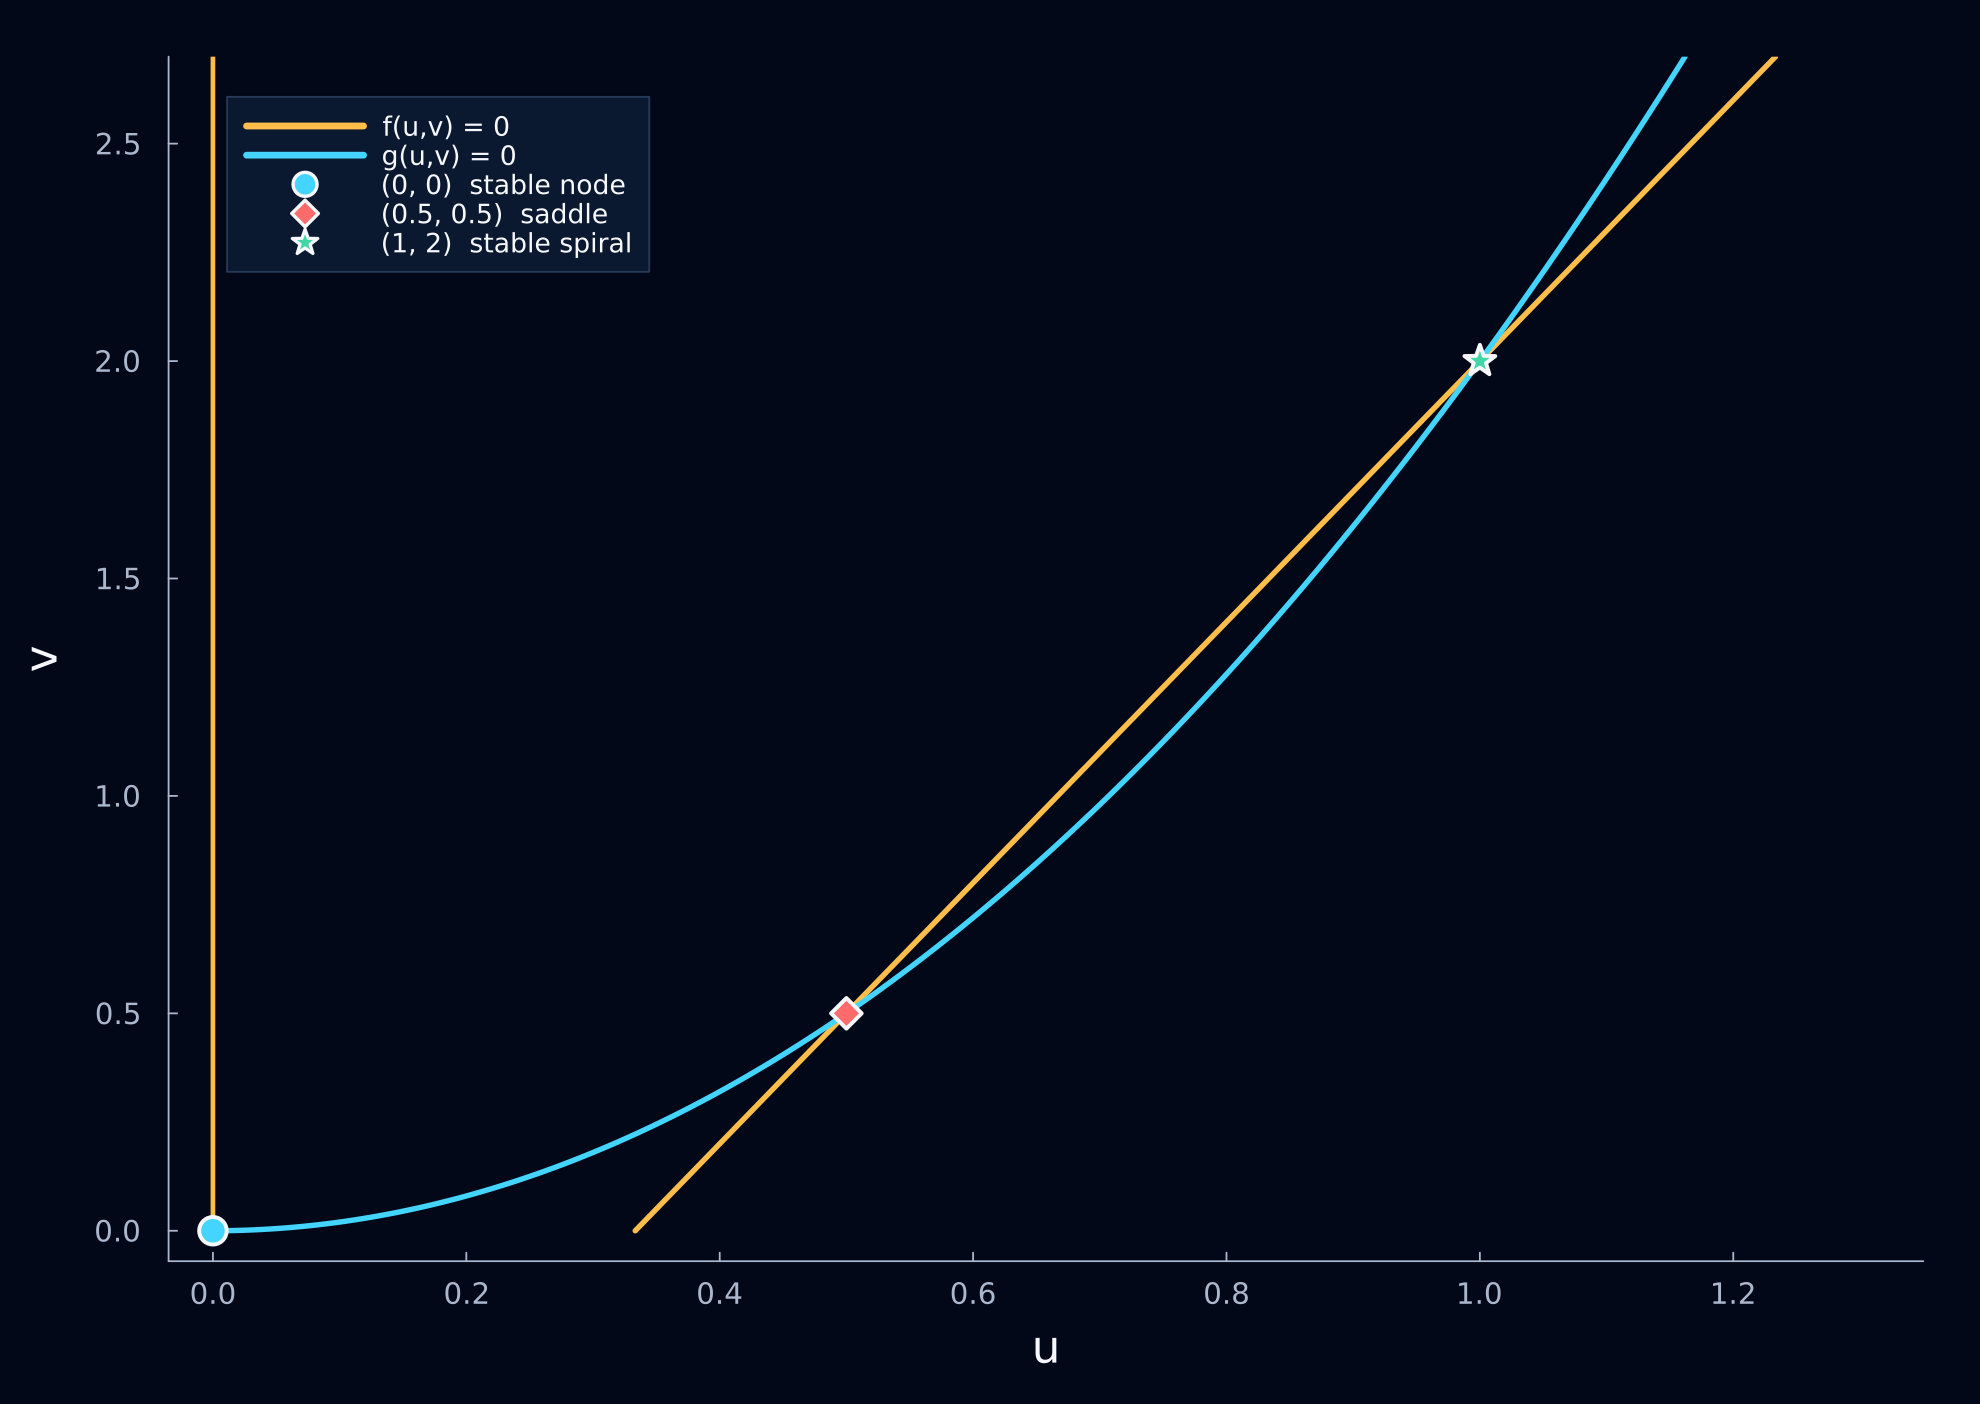
\includegraphics[
        width=\linewidth,
        height=5.20cm,
        keepaspectratio
      ]{figures/D_gierer_meinhardt/gm_example_nullclines.png}

    \end{column}

    \begin{column}{0.28\textwidth}

      \HydraPoint[HydraGold]
        {Activator nullcline}
        {$u=0$ or $v=3u-1$}

      \vspace{0.10cm}

      \HydraPoint[HydraCyan]
        {Inhibitor nullcline}
        {$v=2u^2$}

      \vspace{0.10cm}

      \HydraPoint[HydraGold]
        {Three intersections}
        {Every intersection is a steady state of the local reaction system}

    \end{column}

  \end{columns}

\end{frame}


\begin{frame}{Steady states: local classification}

  \vspace{-0.20cm}

  {\color{HydraMuted}\fontsize{7.7}{9.4}\selectfont
    Evaluate the Jacobian and its eigenvalues at each steady state
  \par}

  \vspace{0.10cm}

  \begin{columns}[T,onlytextwidth]

    \begin{column}{0.31\textwidth}
      \centering

      {\color{HydraWhite}\bfseries\fontsize{10.4}{13.2}\selectfont
      \begin{align*}
        (\bar u,\bar v)
        &=
        (0,0)
      \end{align*}
      }

      \vspace{-0.42cm}

      {\color{HydraWhite}\fontsize{9.1}{11.5}\selectfont
      \begin{align*}
        \lambda_1&=-1
        \\
        \lambda_2&=-0.5
      \end{align*}
      }

      \vspace{-0.34cm}

      \HydraPoint[HydraCyan]
        {Stable node}
        {Both eigenvalues are negative}
    \end{column}

    \begin{column}{0.31\textwidth}
      \centering

      {\color{HydraRed}\bfseries\fontsize{10.4}{13.2}\selectfont
      \begin{align*}
        (\bar u,\bar v)
        &=
        (0.5,0.5)
      \end{align*}
      }

      \vspace{-0.42cm}

      {\color{HydraWhite}\fontsize{9.1}{11.5}\selectfont
      \begin{align*}
        \lambda_-&=-0.72871
        \\
        \lambda_+&=0.22871
      \end{align*}
      }

      \vspace{-0.34cm}

      \HydraPoint[HydraRed]
        {Saddle}
        {One eigenvalue is positive}
    \end{column}

    \begin{column}{0.31\textwidth}
      \centering

      {\color{HydraGreen}\bfseries\fontsize{10.4}{13.2}\selectfont
      \begin{align*}
        (\bar u,\bar v)
        &=
        (1,2)
      \end{align*}
      }

      \vspace{-0.42cm}

      {\color{HydraWhite}\fontsize{9.1}{11.5}\selectfont
      \begin{align*}
        \lambda_\pm
        &=
        -0.25\pm0.32275i
      \end{align*}
      }

      \vspace{-0.00cm}

      \HydraPoint[HydraGreen]
        {Stable spiral}
        {Both real parts are negative}
    \end{column}

  \end{columns}

  \vspace{0.02cm}

  \HydraTakeaway{
    Only the middle steady state has a positive local eigenvalue
  }

\end{frame}


\begin{frame}{Diffusion destabilizes the upper steady state}

  \vspace{-0.26cm}

  \begin{columns}[c,onlytextwidth]

    \begin{column}{0.43\textwidth}

      {\color{HydraMuted}\fontsize{7.6}{9.3}\selectfont
        Linearization at the stable steady state $(1,2)$
      \par}

      \vspace{-0.28cm}

      {\color{HydraWhite}\fontsize{9.5}{12}\selectfont
      \begin{align*}
        J(1,2)
        &=
        \begin{pmatrix}
          0.5&-1/6
          \\
          4&-1
        \end{pmatrix}
        \\
        \operatorname{tr}J(1,2)
        &=
        -0.5
        \\
        \det J(1,2)
        &=
        \frac{1}{6}
      \end{align*}
      }

    \end{column}

    \begin{column}{0.53\textwidth}

      {\color{HydraWhite}\fontsize{9.2}{11.7}\selectfont
      \begin{align*}
        M_k
        &=
        \begin{pmatrix}
          0.5-0.01\mu_k&-1/6
          \\
          4&-1-\mu_k
        \end{pmatrix}
        \\
        \det(M_k)
        &=
        \frac{1}{6}
        -
        0.49\mu_k
        +
        0.01\mu_k^2
      \end{align*}
      }

    \end{column}

  \end{columns}

  \vspace{-0.34cm}

  {\color{HydraGold}\bfseries\fontsize{11.4}{14.4}\selectfont
  \begin{align*}
    \boxed{
      \det(M_k)<0
      \quad\Longleftrightarrow\quad
      0.34253<\mu_k<48.65747
    }
  \end{align*}
  }

  \vspace{-0.30cm}

  \HydraTakeaway{
    Modes whose Laplacian eigenvalues lie inside this interval are unstable
  }

\end{frame}


\begin{frame}{Unstable eigenmodes}

  \vspace{-0.20cm}

  \begin{columns}[c,onlytextwidth]

    \begin{column}{0.70\textwidth}
      \centering

      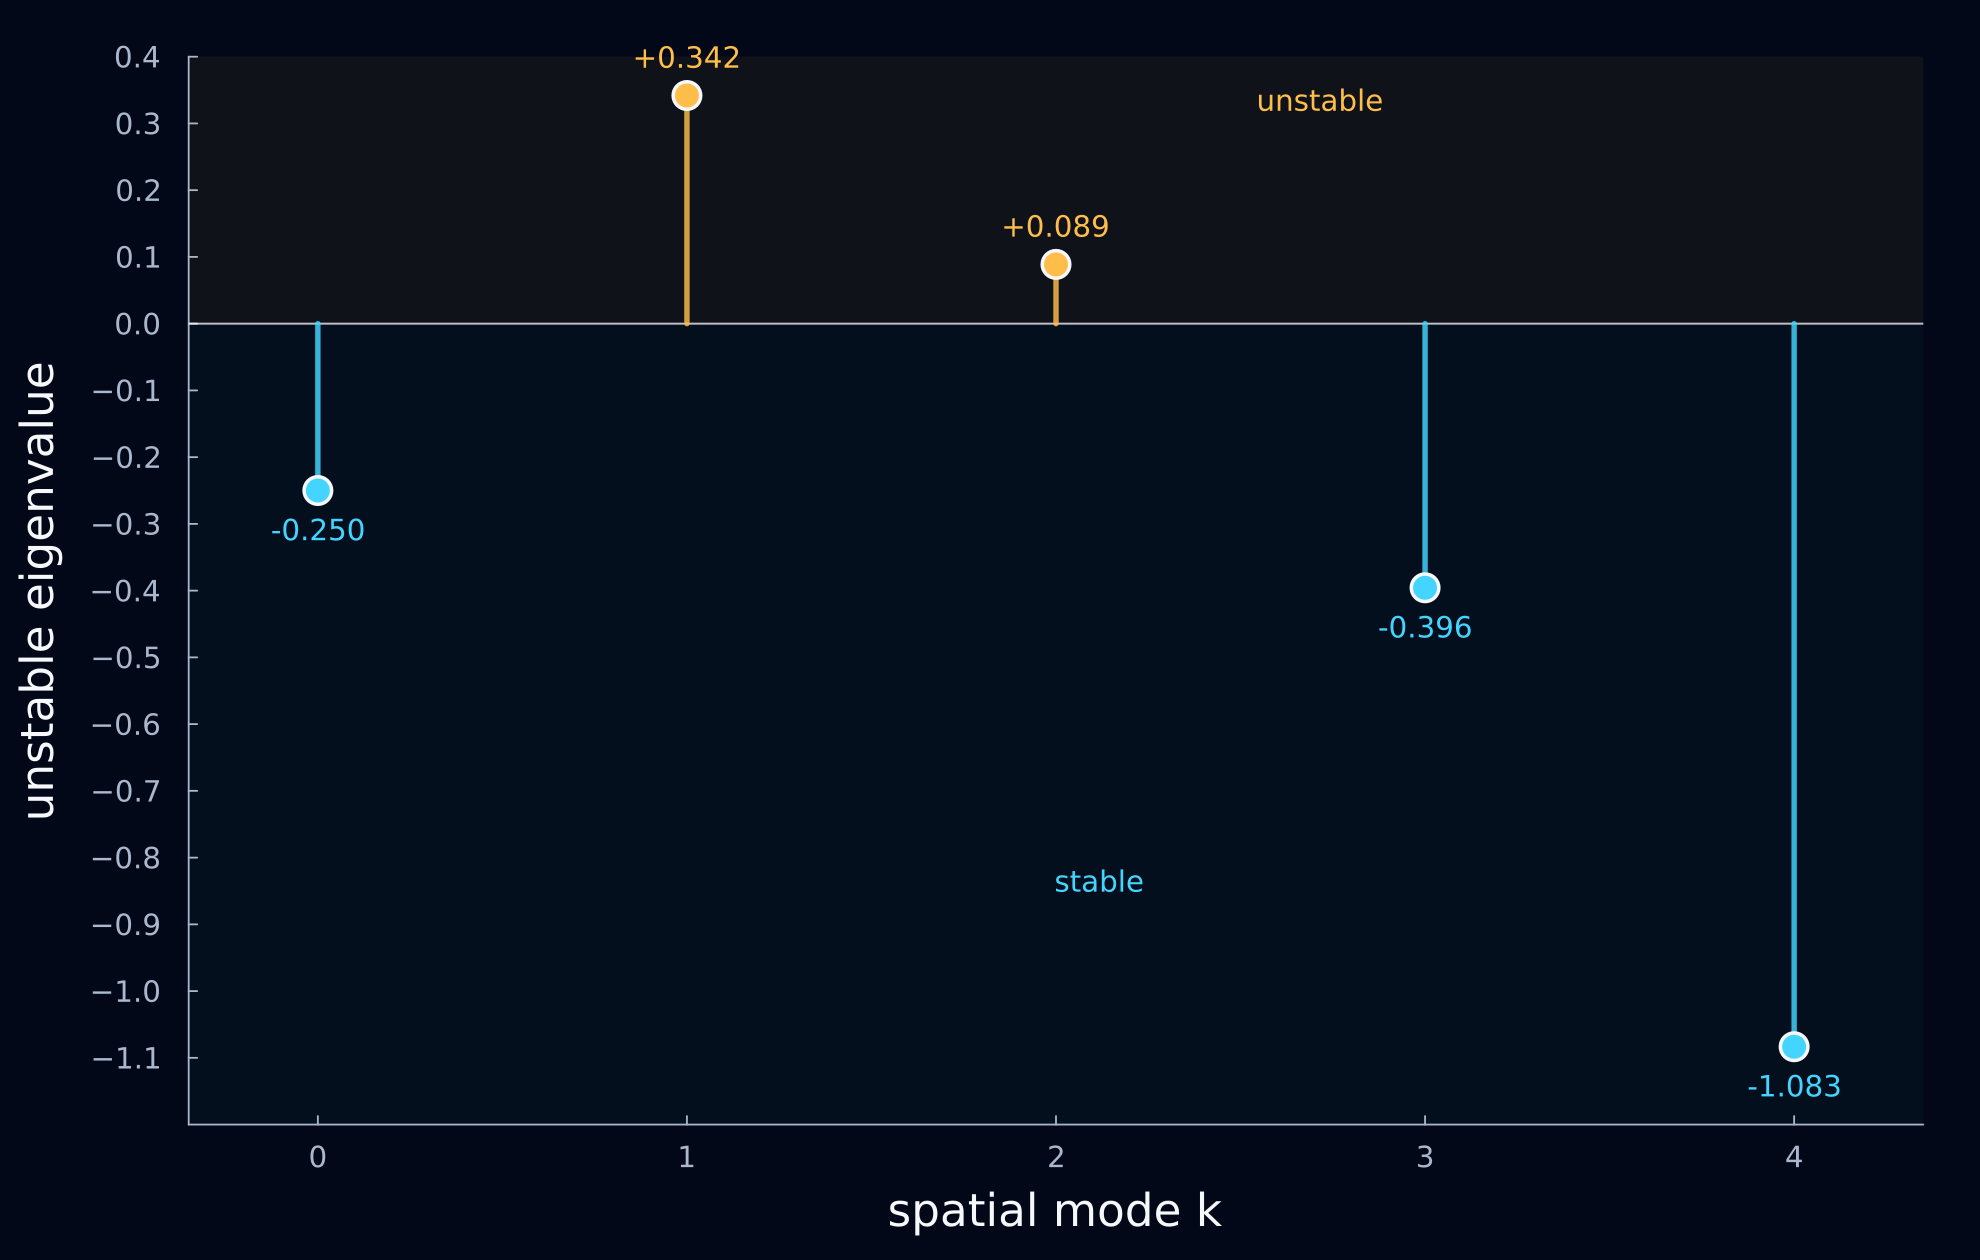
\includegraphics[
        width=\linewidth,
        height=5.10cm,
        keepaspectratio
      ]{figures/D_gierer_meinhardt/gm_example_mode_growth_rates.png}

    \end{column}

    \begin{column}{0.26\textwidth}

      {\color{HydraMuted}\fontsize{7.4}{9.1}\selectfont
        $D_u=0.01$ \quad $D_v=1$ \quad $L=1$
      \par}

      \vspace{0.18cm}

      \HydraPoint[HydraGold]
        {Dominant mode $k=1$}
        {$\lambda_{1,+}=0.34184$}

      \vspace{-0.04cm}

      \HydraPoint[HydraGold]
        {Slower mode $k=2$}
        {$\lambda_{2,+}=0.08878$}

      \vspace{-0.04cm}

      \HydraPoint[HydraCyan]
        {Stable neighbors}
        {$k=0,3,...$ decay}

    \end{column}

  \end{columns}

\end{frame}


\begin{frame}{The first five spatial eigenmodes on $\Omega=[0,1]$}

  \vspace{-0.34cm}

  \begin{columns}[c,onlytextwidth]

    \begin{column}{0.56\textwidth}
      {\color{HydraMuted}\fontsize{7.5}{9.2}\selectfont
        Steady states of the local reaction system
      \par}

      \vspace{-0.36cm}

      {\color{HydraWhite}\fontsize{9.0}{11.4}\selectfont
      \begin{align*}
        {\color{HydraWhite}(0,0)}
        \qquad
        {\color{HydraRed}(0.5,0.5)}
        \qquad
        {\color{HydraGreen}(1,2)}
      \end{align*}
      }
    \end{column}

    \begin{column}{0.40\textwidth}
      {\color{HydraGold}\bfseries\fontsize{7.5}{9.2}\selectfont
        LINEARIZATION USED BELOW\par}

      \vspace{-0.36cm}

      {\color{HydraWhite}\bfseries\fontsize{9.2}{11.7}\selectfont
      \begin{align*}
        (\bar u,\bar v)={\color{HydraGreen}(1,2)}
      \end{align*}
      }
    \end{column}

  \end{columns}

  \vspace{-0.40cm}

  {\color{HydraWhite}\fontsize{8.8}{11.1}\selectfont
  \begin{align*}
    \phi_k(x)
    &=
    \cos(k\pi x)
    &
    \rho_k
    &=
    \max_{\lambda\in\sigma(M_k)}\operatorname{Re}\lambda
  \end{align*}
  }

  \vspace{-0.48cm}

  \begin{columns}[c,onlytextwidth]

    \begin{column}{0.68\textwidth}
      {\color{HydraWhite}\fontsize{7.2}{9.0}\selectfont
      \begin{align*}
        \begin{array}{c@{\hspace{0.25cm}}c@{\hspace{0.32cm}}r@{\hspace{0.28cm}}l}
          k
          &
          \phi_k(x)
          &
          \rho_k
          &
          \text{behavior}
          \\[0.08cm]
          1
          &
          \cos(\pi x)
          &
          {\color{HydraGold}+0.34184}
          &
          \textcolor{HydraGold}{\text{unstable}}
          \\
          2
          &
          \cos(2\pi x)
          &
          {\color{HydraGold}+0.08878}
          &
          \textcolor{HydraGold}{\text{unstable}}
          \\
          3
          &
          \cos(3\pi x)
          &
          {\color{HydraCyan}-0.39572}
          &
          \textcolor{HydraCyan}{\text{stable}}
          \\
          4
          &
          \cos(4\pi x)
          &
          {\color{HydraCyan}-1.08336}
          &
          \textcolor{HydraCyan}{\text{stable}}
          \\
          5
          &
          \cos(5\pi x)
          &
          {\color{HydraCyan}-1.97011}
          &
          \textcolor{HydraCyan}{\text{stable}}
        \end{array}
      \end{align*}
      }
    \end{column}

    \begin{column}{0.28\textwidth}
      \centering

      {\color{HydraGold}\bfseries\fontsize{7.2}{8.8}\selectfont
        DOMINANT UNSTABLE MODE\par}

      \vspace{0.08cm}

      \begin{tikzpicture}[x=3.05cm,y=0.78cm]
        \draw[-{Latex[length=1.8mm]},HydraMuted,line width=0.65pt]
          (-0.04,0) -- (1.10,0)
          node[below,text=HydraMuted,font=\fontsize{6.5}{7.8}\selectfont] {$x$};
        \draw[-{Latex[length=1.8mm]},HydraMuted,line width=0.65pt]
          (0,-1.25) -- (0,1.32);

        \draw[HydraGold,line width=1.55pt,domain=0:1,samples=100]
          plot (\x,{cos(180*\x)});

        \node[anchor=north,text=HydraMuted,
          font=\fontsize{6.2}{7.4}\selectfont]
          at (0,-0.08) {$0$};
        \node[anchor=north,text=HydraMuted,
          font=\fontsize{6.2}{7.4}\selectfont]
          at (1,-0.08) {$1$};
      \end{tikzpicture}

      \vspace{-0.06cm}

      {\color{HydraWhite}\fontsize{7.4}{9.2}\selectfont
        $\phi_1(x)=\cos(\pi x)$
      \par}
    \end{column}

  \end{columns}

\end{frame}

\begin{frame}{Unstable eigenmodes on a larger domain $\Omega=[0,10]$}

  \vspace{-0.20cm}

  \begin{columns}[c,onlytextwidth]

    \begin{column}{0.70\textwidth}
      \centering

      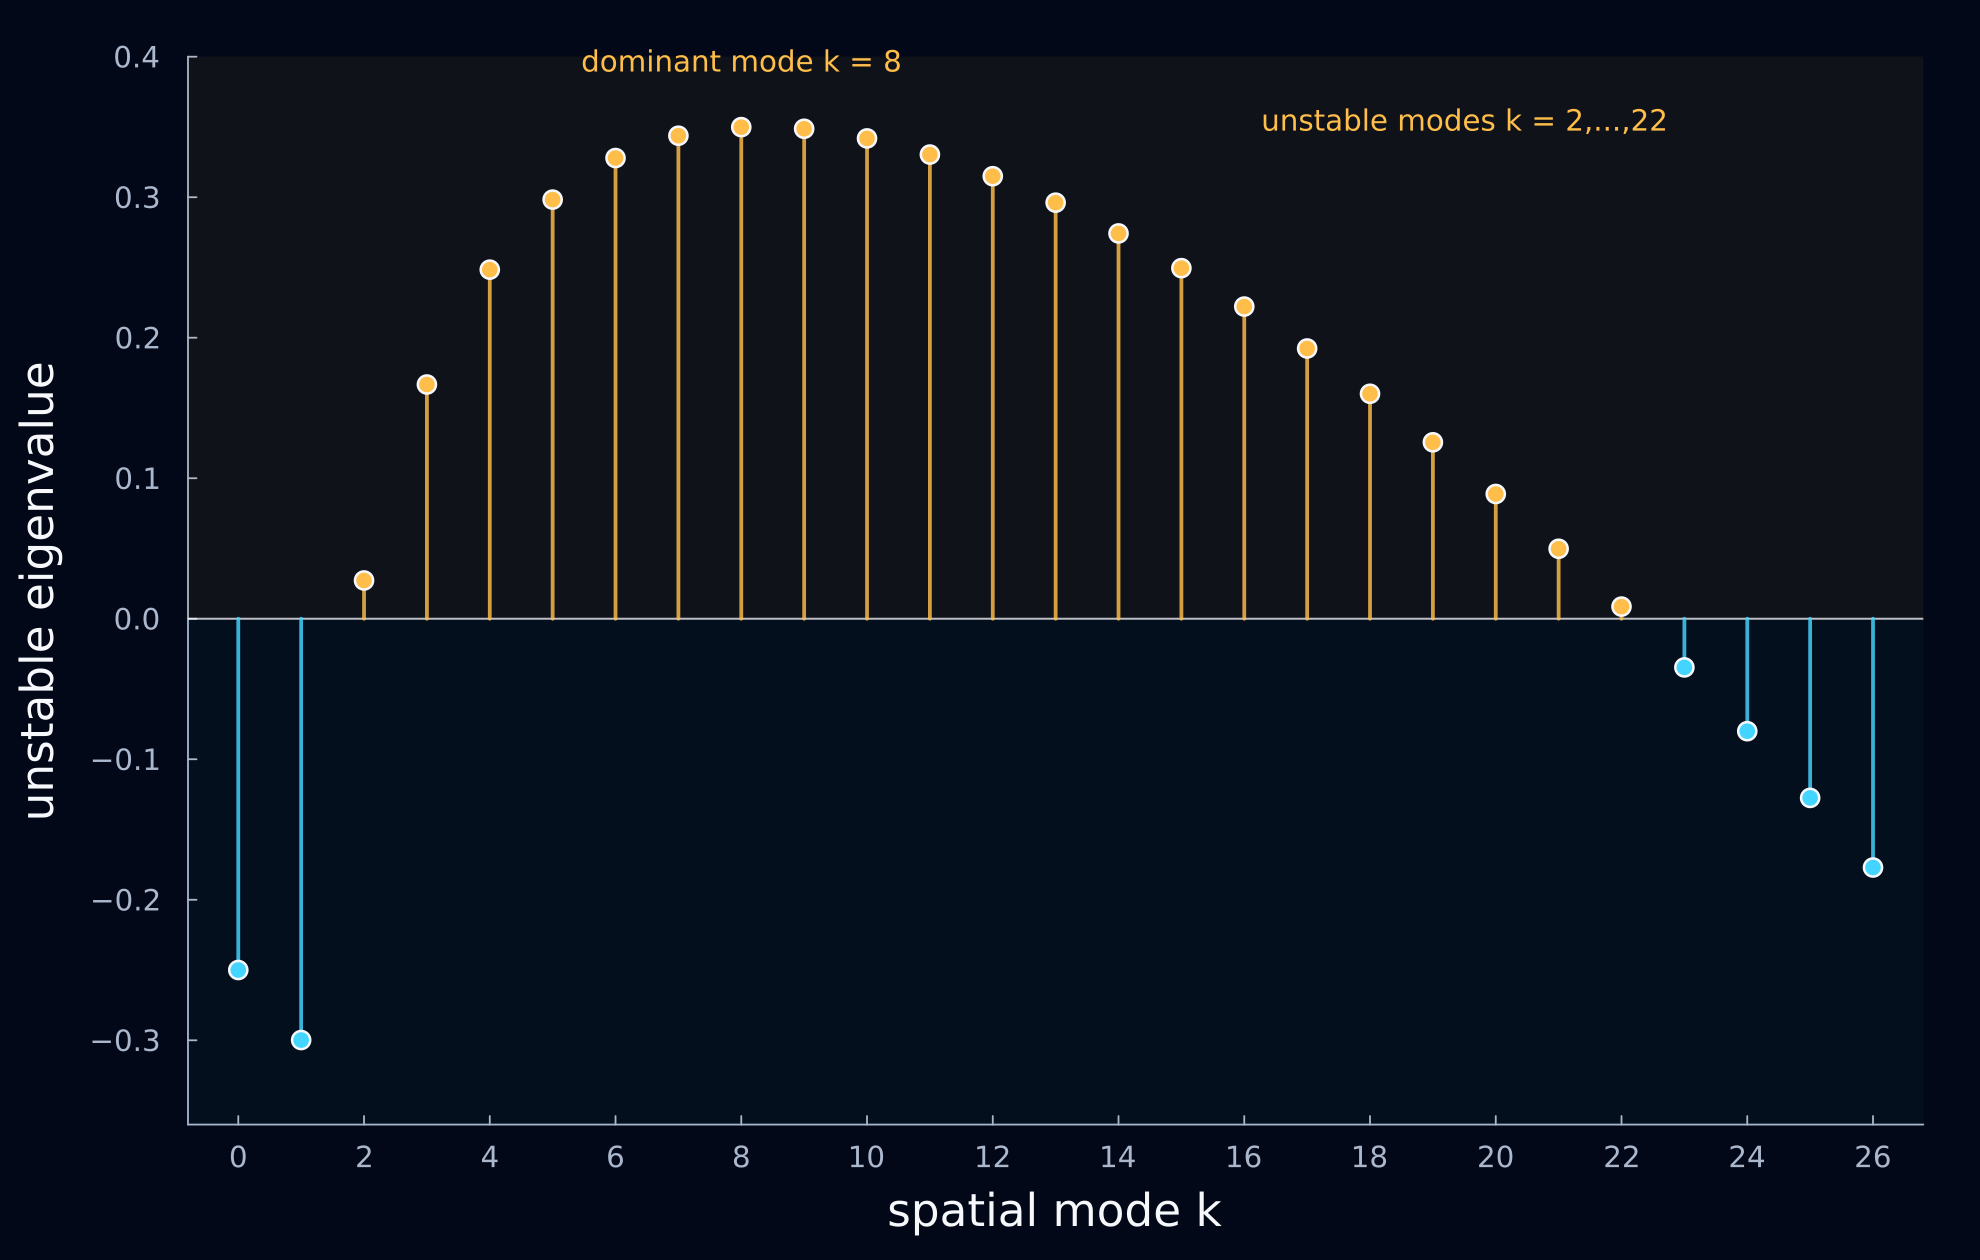
\includegraphics[
        width=\linewidth,
        height=5.10cm,
        keepaspectratio
      ]{figures/D_gierer_meinhardt/gm_example_mode_growth_rates_L10.png}

    \end{column}

    \begin{column}{0.26\textwidth}

      {\color{HydraMuted}\fontsize{7.4}{9.1}\selectfont
        $D_u=0.01$, \quad $D_v=1$, \quad $L=10$
      \par}

      \vspace{0.18cm}

      \HydraPoint[HydraGold]
        {Many unstable modes}
        {$k=2,\ldots,22$}

      \vspace{-0.04cm}

      \HydraPoint[HydraGold]
        {Dominant mode $k=8$}
        {$\lambda_{8,+}=0.34988$}

      \vspace{-0.04cm}

      \HydraPoint[HydraCyan]
        {Stable neighbors}
        {$k=0,1,23,...$ decay}

    \end{column}

  \end{columns}

  \vspace{0.36cm}

  \HydraTakeaway{
    The longer domain places more discrete eigenvalues inside the same unstable band
  }

\end{frame}

\begin{frame}{Selected spatial eigenmodes on $\Omega=[0,10]$}

  \vspace{-0.34cm}

  \begin{columns}[c,onlytextwidth]

    \begin{column}{0.56\textwidth}



      {\color{HydraWhite}\fontsize{9.0}{11.4}\selectfont
      \begin{align*}
        {\color{HydraWhite}(0,0)}
        \qquad
        {\color{HydraRed}(0.5,0.5)}
        \qquad
        {\color{HydraGreen}(1,2)}
      \end{align*}
      }
    \end{column}

    \begin{column}{0.40\textwidth}


      \vspace{-0.36cm}

      {\color{HydraWhite}\bfseries\fontsize{9.2}{11.7}\selectfont
      \begin{align*}
        (\bar u,\bar v)={\color{HydraGreen}(1,2)}
      \end{align*}
      }
    \end{column}

  \end{columns}

  \vspace{-0.40cm}

  {\color{HydraWhite}\fontsize{8.8}{11.1}\selectfont
  \begin{align*}
    \phi_k(x)
    &=
    \cos\!\left(\frac{k\pi x}{10}\right)
    &
    \rho_k
    &=
    \max_{\lambda\in\sigma(M_k)}\operatorname{Re}\lambda
  \end{align*}
  }

  \vspace{-0.48cm}

  \begin{columns}[c,onlytextwidth]

    \begin{column}{0.72\textwidth}
      {\color{HydraWhite}\fontsize{6.5}{7.8}\selectfont
      \renewcommand{\arraystretch}{0.86}
      \begin{align*}
        \begin{array}{c@{\hspace{0.16cm}}c@{\hspace{0.22cm}}r@{\hspace{0.20cm}}l}
      k
      &
      \phi_k(x)
      &
      \rho_k
      &
      \text{behavior}
      \\[0.08cm]
      1
      &
      \cos(\pi x/10)
      &
      {\color{HydraCyan}-0.29984}
      &
      \textcolor{HydraCyan}{\text{stable}}
      \\
      2
      &
      \cos(2\pi x/10)
      &
      {\color{HydraGold}+0.02724}
      &
      \textcolor{HydraGold}{\text{unstable}}
      \\
      \vdots
      &
      \vdots
      &
      \vdots
      &
      \\
      6
      &
      \cos(6\pi x/10)
      &
      {\color{HydraGold}+0.32788}
      &
      \textcolor{HydraGold}{\text{unstable}}
      \\
      7
      &
      \cos(7\pi x/10)
      &
      {\color{HydraGold}+0.34376}
      &
      \textcolor{HydraGold}{\text{unstable}}
      \\
      {\color{HydraGold}\mathbf{8}}
      &
      {\color{HydraGold}\cos(8\pi x/10)}
      &
      {\color{HydraGold}\mathbf{+0.34988}}
      &
      \textcolor{HydraGold}{\text{unstable}}
      \\
      9
      &
      \cos(9\pi x/10)
      &
      {\color{HydraGold}+0.34870}
      &
      \textcolor{HydraGold}{\text{unstable}}
      \\
      10
      &
      \cos(10\pi x/10)
      &
      {\color{HydraGold}+0.34184}
      &
      \textcolor{HydraGold}{\text{unstable}}
      \\
      \vdots
      &
      \vdots
      &
      \vdots
      &
      \\
      21
      &
      \cos(21\pi x/10)
      &
      {\color{HydraGold}+0.04979}
      &
      \textcolor{HydraGold}{\text{unstable}}
      \\
      22
      &
      \cos(22\pi x/10)
      &
      {\color{HydraGold}+0.00864}
      &
      \textcolor{HydraGold}{\text{unstable}}
      \\
      23
      &
      \cos(23\pi x/10)
      &
      {\color{HydraCyan}-0.03464}
      &
      \textcolor{HydraCyan}{\text{stable}}
        \end{array}
      \end{align*}
      }
    \end{column}

    \begin{column}{0.24\textwidth}
      \centering

      {\color{HydraGold}\bfseries\fontsize{6.8}{8.3}\selectfont
        DOMINANT UNSTABLE MODE\par}

      \vspace{0.08cm}

      \begin{tikzpicture}[x=0.265cm,y=0.68cm]
        \draw[-{Latex[length=1.7mm]},HydraMuted,line width=0.62pt]
          (-0.4,0) -- (11.2,0)
          node[below,text=HydraMuted,font=\fontsize{6.2}{7.4}\selectfont]
          {$x$};
        \draw[-{Latex[length=1.7mm]},HydraMuted,line width=0.62pt]
          (0,-1.28) -- (0,1.34);

        \draw[HydraGold,line width=1.40pt,domain=0:10,samples=180]
          plot (\x,{cos(144*\x)});

        \node[anchor=north,text=HydraMuted,
          font=\fontsize{6}{7.2}\selectfont]
          at (0,-0.10) {$0$};
        \node[anchor=north,text=HydraMuted,
          font=\fontsize{6}{7.2}\selectfont]
          at (10,-0.10) {$10$};
      \end{tikzpicture}

      \vspace{-0.06cm}

      {\color{HydraWhite}\fontsize{6.8}{8.5}\selectfont
        $\phi_8(x)=\cos\!\left(\dfrac{8\pi x}{10}\right)$
      \par}
    \end{column}

  \end{columns}


\end{frame} 


% \begin{frame}{Turing analysis predicts onset but not the final pattern}

%   \vspace{-0.18cm}

%   \begin{columns}[c,onlytextwidth]

%     \begin{column}{0.65\textwidth}
%       \centering

%       % REPLACEABLE VISUAL
%       % Replace the tikzpicture with:
%       % \includegraphics[width=\linewidth,height=5.10cm,keepaspectratio]{figures/D_gierer_meinhardt/linear_to_nonlinear.png}
%       \begin{tikzpicture}[x=0.90cm,y=0.90cm]
%         \node[text=HydraGold,font=\bfseries\fontsize{7.5}{9}\selectfont]
%           at (2.45,4.95) {early linear growth};
%         \node[text=HydraCyan,font=\bfseries\fontsize{7.5}{9}\selectfont]
%           at (7.95,4.95) {final nonlinear state};

%         \draw[-{Latex[length=1.9mm]},HydraMuted,line width=0.7pt]
%           (0.35,2.35) -- (4.65,2.35);
%         \draw[-{Latex[length=1.9mm]},HydraMuted,line width=0.7pt]
%           (5.75,2.35) -- (10.35,2.35);

%         \draw[HydraGold,line width=1.55pt,domain=0:4.1,samples=100]
%           plot ({0.45+\x},{2.35+0.55*cos(180*\x)});

%         \draw[HydraCyan,line width=1.65pt]
%           plot[smooth] coordinates {
%             (5.90,2.36) (6.35,2.40) (6.75,2.72) (6.95,4.30)
%             (7.15,2.70) (7.55,2.38) (8.05,2.40) (8.45,2.58)
%             (8.62,3.58) (8.82,2.58) (9.25,2.38) (10.20,2.36)
%           };

%         \draw[-{Latex[length=2.6mm]},HydraWhite,line width=1.1pt]
%           (4.75,3.35) -- (5.55,3.35);
%         \node[text=HydraMuted,font=\fontsize{6.8}{8.2}\selectfont,
%           align=center]
%           at (5.15,2.78) {nonlinear\\evolution};

%         \node[text=HydraMuted,font=\fontsize{7}{8.5}\selectfont,
%           align=center,text width=3.6cm]
%           at (2.45,0.95) {linear theory identifies which small perturbations initially grow};
%         \node[text=HydraMuted,font=\fontsize{7}{8.5}\selectfont,
%           align=center,text width=4.0cm]
%           at (8.10,0.95) {peak amplitudes and the final shape emerge far from the steady state};
%       \end{tikzpicture}

%     \end{column}

%     \begin{column}{0.31\textwidth}

%       \HydraPoint[HydraGold]
%         {Linear level}
%         {Turing analysis describes infinitesimal perturbations near $(u_+,v_+)$}

%       \vspace{-0.04cm}

%       \HydraPoint[HydraCyan]
%         {Nonlinear pattern formation}
%         {Domain size, initial conditions and competition between peaks affect the outcome}

%       \vspace{-0.04cm}

%       \HydraPoint[HydraGold]
%         {Useful but incomplete}
%         {Unstable eigenmodes can help predict a pattern but do not give a complete description}

%     \end{column}

%   \end{columns}

%   \vspace{-0.18cm}

%   \HydraTakeaway{
%     Growth, division and wounds can move the system far from the state analysed by linear theory
%   }

% \end{frame}
